\chapter{Inserimento guasti e Rilevamento}

Nella prima fase del nostro studio, abbiamo implementato una strategia di rilevamento del guasto al motore mediante la modifica dei valori PWM utilizzando Simulink. Questo è stato eseguito nel blocco "Quadcopter Model" nel file Simulink "UAV Dynamics" (Figura \ref{fig:guasto PWM}).
\begin{figure}[H]  % 'H' forza la posizione esatta
    \centering
    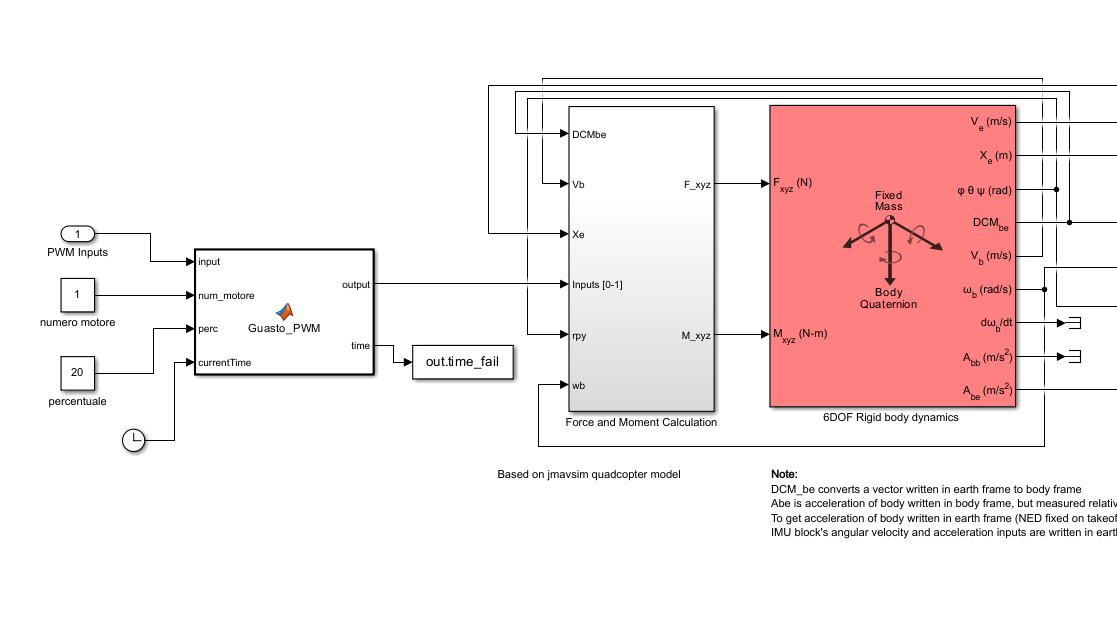
\includegraphics[width=0.8\textwidth]{guasto_pwm.png}
    \caption{Blocco Guasto PWM}
    \label{fig:guasto PWM}
\end{figure}
\noindent
Abbiamo introdotto una funzione MATLAB all'interno del blocco "matlab\_function", la quale prende in input il numero del motore interessato, la percentuale di guasto da applicare al PWM e il tempo corrente.

\begin{lstlisting}[language=Matlab, caption={Funzione MATLAB per il rilevamento del guasto PWM}, label=lst:guasto_pwm]
function [output, time] = Guasto_PWM(input, num_motore, 
perc, currentTime)   
    if num_motore == 0
        output = input;
        time = 0;
    else
        % Copia i valori di PWM in una variabile temporanea
        output = input;
        % Diminuisci il % del valore del PWM del motore 
        specificato
        output(num_motore) = (100 - perc) / 100 * 
        output(num_motore);
        % Ottieni istante inserimento guasto
        time = currentTime;
    end
end
\end{lstlisting}
\noindent

Nella funzione mostrata nel listato~\ref{lst:guasto_pwm}, consente di simulare il guasto riducendo la percentuale di PWM del motore specificato. 

\begin{figure}[H]  % 'H' forza la posizione esatta
    \centering
    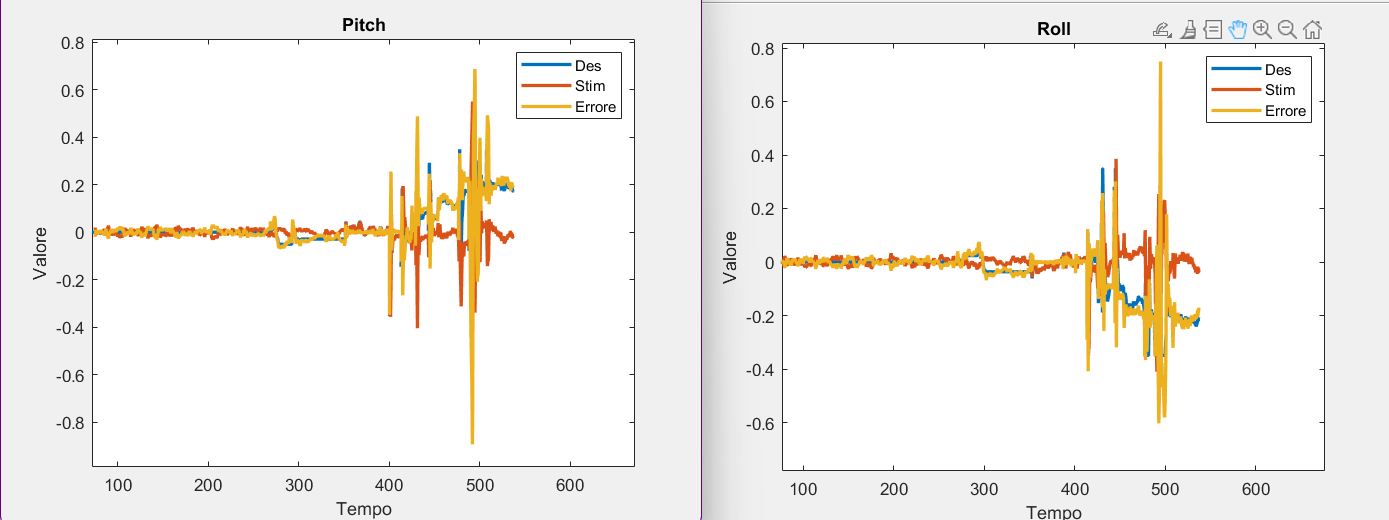
\includegraphics[width=0.9\textwidth]{pitch_roll.png}
    \caption{Andamento Angoli di Eulero Pitch e Roll con guasto al 20\% sul PWM del motore 1}
    \label{fig:pitch_roll}
\end{figure}

\noindent
Dopo aver introdotto un guasto in uno dei motori durante il volo del drone e aver eseguito una curva, abbiamo notato che l'errore tra gli angoli desiderati e stimati di pitch e roll assumeva valori diversi da zero (Figura \ref{fig:pitch_roll}). 
\noindent
Questa osservazione ha costituito la base per lo sviluppo degli algoritmi di rilevamento del guasto successivi.

\section{Rilevamento dei Guasti tramite Soglia Fissa}

Nella fase successiva del nostro studio, ci siamo concentrati sullo sviluppo di un algoritmo di rilevamento dei guasti tramite soglia fissa. Questo approccio si basa sull'osservazione della variazione dell'errore degli angoli di pitch e roll dopo l'inserimento di un guasto su uno dei motori del drone. L'errore era calcolato confrontando l'angolo desiderato con quello stimato (eq. \ref{eq:pitch_error} ed eq. \ref{eq:roll_error}) . Abbiamo notato che questa variazione dipendeva dal motore interessato dal guasto.
\begin{equation}
\text{Errore di pitch} = \text{Angolo desiderato di pitch} - \text{Angolo stimato di pitch}
\label{eq:pitch_error}
\end{equation}
\begin{equation}
\text{Errore di roll} = \text{Angolo desiderato di roll} - \text{Angolo stimato di roll}
\label{eq:roll_error}
\end{equation}
\noindent
La rilevazione dei guasti avviente dentro al FlightController, quindi all'interno del file Simulink "Quadcopter\_ControllerWithNavigation" sono stati inseriti i seguenti blocchi mostrati in figura \ref{fig:Blocchi per il rilevamento a soglia fissa con buffer}.

\begin{figure}[H]  % 'H' forza la posizione esatta
    \centering
    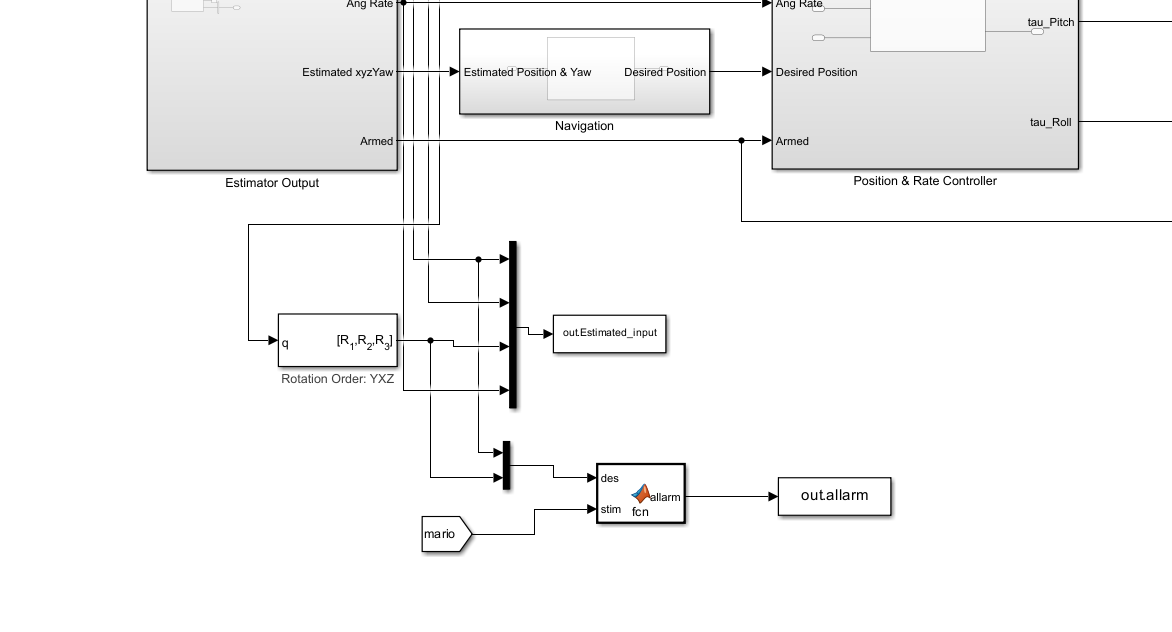
\includegraphics[width=0.9\textwidth]{files/images/soglia_fissa_buffer.png}
    \caption{Blocchi per il rilevamento a soglia fissa con buffer in Quadcopter\_ControllerWithNavigation}
    \label{fig:Blocchi per il rilevamento a soglia fissa con buffer}
\end{figure}
\noindent
Per implementare l'algoritmo di rilevamento dei guasti, abbiamo definito delle soglie fisse sugli errori degli angoli di pitch e roll. Durante la fase di volo del drone, abbiamo monitorato costantemente gli errori degli angoli di pitch e roll e abbiamo confrontato i loro valori con le soglie fissate. Quando entrambi gli errori di  dei valori superava la soglia prestabilita, scattava un allarme indicando il motore affetto dal guasto.
\\
Per aumentare l'efficienza del rilevamento, abbiamo utilizzato un buffer di campionamento. Ogni volta che veniva rilevata una variazione sugli angoli di pitch e roll, registravamo i valori degli angoli per un numero prefissato di campioni, ad esempio 500 (equivale ad un campionamento di 5 secondi). Successivamente, calcolavamo la media degli angoli registrati e confrontavamo questa media con le soglie fisse. Se la media superava una delle soglie, l'allarme di guasto veniva attivato. Il seguente è il codice all'interno del blocco funzione MATLAB, mostrato in figura \ref{fig:Blocchi per il rilevamento a soglia fissa con buffer}, per la rilevazione guasti.
\begin{lstlisting}[language=Matlab, caption={Descrizione del codice}, label={lst:codice_matlab}]
function allarm = fcn(stim, des)
    persistent PitchBuffer RollBuffer
    if isempty(PitchBuffer)
        PitchBuffer = zeros(1, 500);
        RollBuffer = zeros(1, 500);
    end

    % Calcolo gli errori di Pitch e Roll
    Pitch_Error = des(2) - stim(2);
    Roll_Error = des(3) - stim(3);

    % Per evitare che la media dia errore per i NaN, 
    sostituisco con 0
    if(isnan(Pitch_Error) && isnan(Roll_Error))
       Pitch_Error = 0;
       Roll_Error = 0;
    end

    % Aggiorna i buffer
    PitchBuffer = [PitchBuffer(2:end), Pitch_Error];
    RollBuffer = [RollBuffer(2:end), Roll_Error];

    % Soglie fisse
    PitchThreshold = 0.1;
    RollThreshold = 0.1;

    % Guasto Motore 1 del -20%
    if (mean(PitchBuffer) > PitchThreshold && 
    mean(RollBuffer) < -RollThreshold)
        allarm = 1;
    % Guasto Motore 2 del -20%
    elseif (mean(PitchBuffer) < -PitchThreshold && 
    mean(RollBuffer) > RollThreshold)
        allarm = 2;
    % Guasto Motore 3 del -20%
    elseif (mean(PitchBuffer) > PitchThreshold && 
    mean(RollBuffer) > RollThreshold)
        allarm = 3;
    % Guasto Motore 4 del -20%
    elseif (mean(PitchBuffer) < -PitchThreshold && 
    mean(RollBuffer) < -RollThreshold)
        allarm = 4;
    else
        allarm = 0;
    end
end
\end{lstlisting}
\noindent
Abbiamo osservato che l'approccio di rilevamento dei guasti tramite soglia fissa si è dimostrato efficace nel rilevare guasti durante la prima curva effettuata dal drone.
\\
Il percorso utilizzato per il test di volo con rilevamento guasto a soglia fissa è mostrato in Figura \ref{fig:Percorso Test Soglia Fissa con Buffer}. Durante ogni volo, il guasto è stato inserito tra il punto 7 e il punto 8 del percorso. Si sono ottenuti risultati distinti inserendo il guasto su ciascun motore durante i test.

\begin{figure}[H]
    \centering
    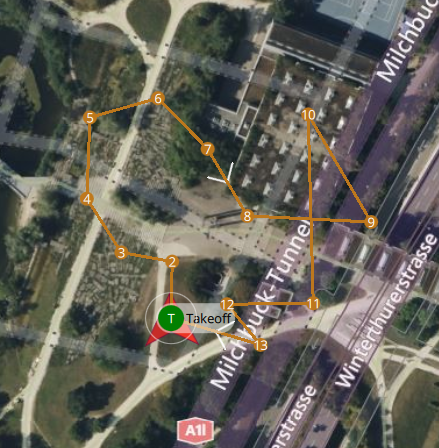
\includegraphics[width=0.5\textwidth]{files/images/path_soglia_fissa1 (1).png}
    \caption{Percorso Test Soglia Fissa con Buffer}
    \label{fig:Percorso Test Soglia Fissa con Buffer}
\end{figure}
\noindent
Ogni test ha prodotto risultati soddisfacenti, poiché non sono stati riscontrati falsi positivi e i falsi negativi sono stati osservati solamente nel tratto compreso tra l'inserimento del guasto e la prima curva da effettuare.

\begin{figure}[H]
    \centering
    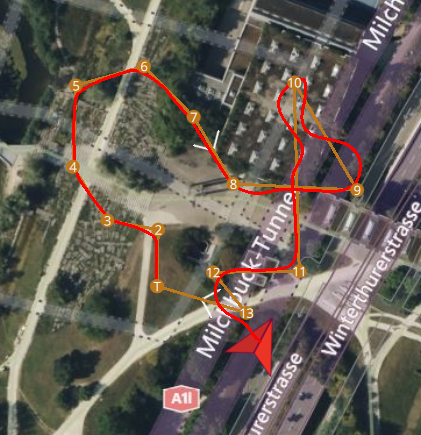
\includegraphics[width=0.5\textwidth]{files/images/path_soglia_fissa1 (2).png}
    \caption{Andamento del drone del test volo con guasto su potenza motore del 20\% su motore 1}
    \label{Risultato volo con guasto su potenza motore del 20\% su motore 1}
\end{figure}
\noindent

\begin{figure}[H]
    \centering
    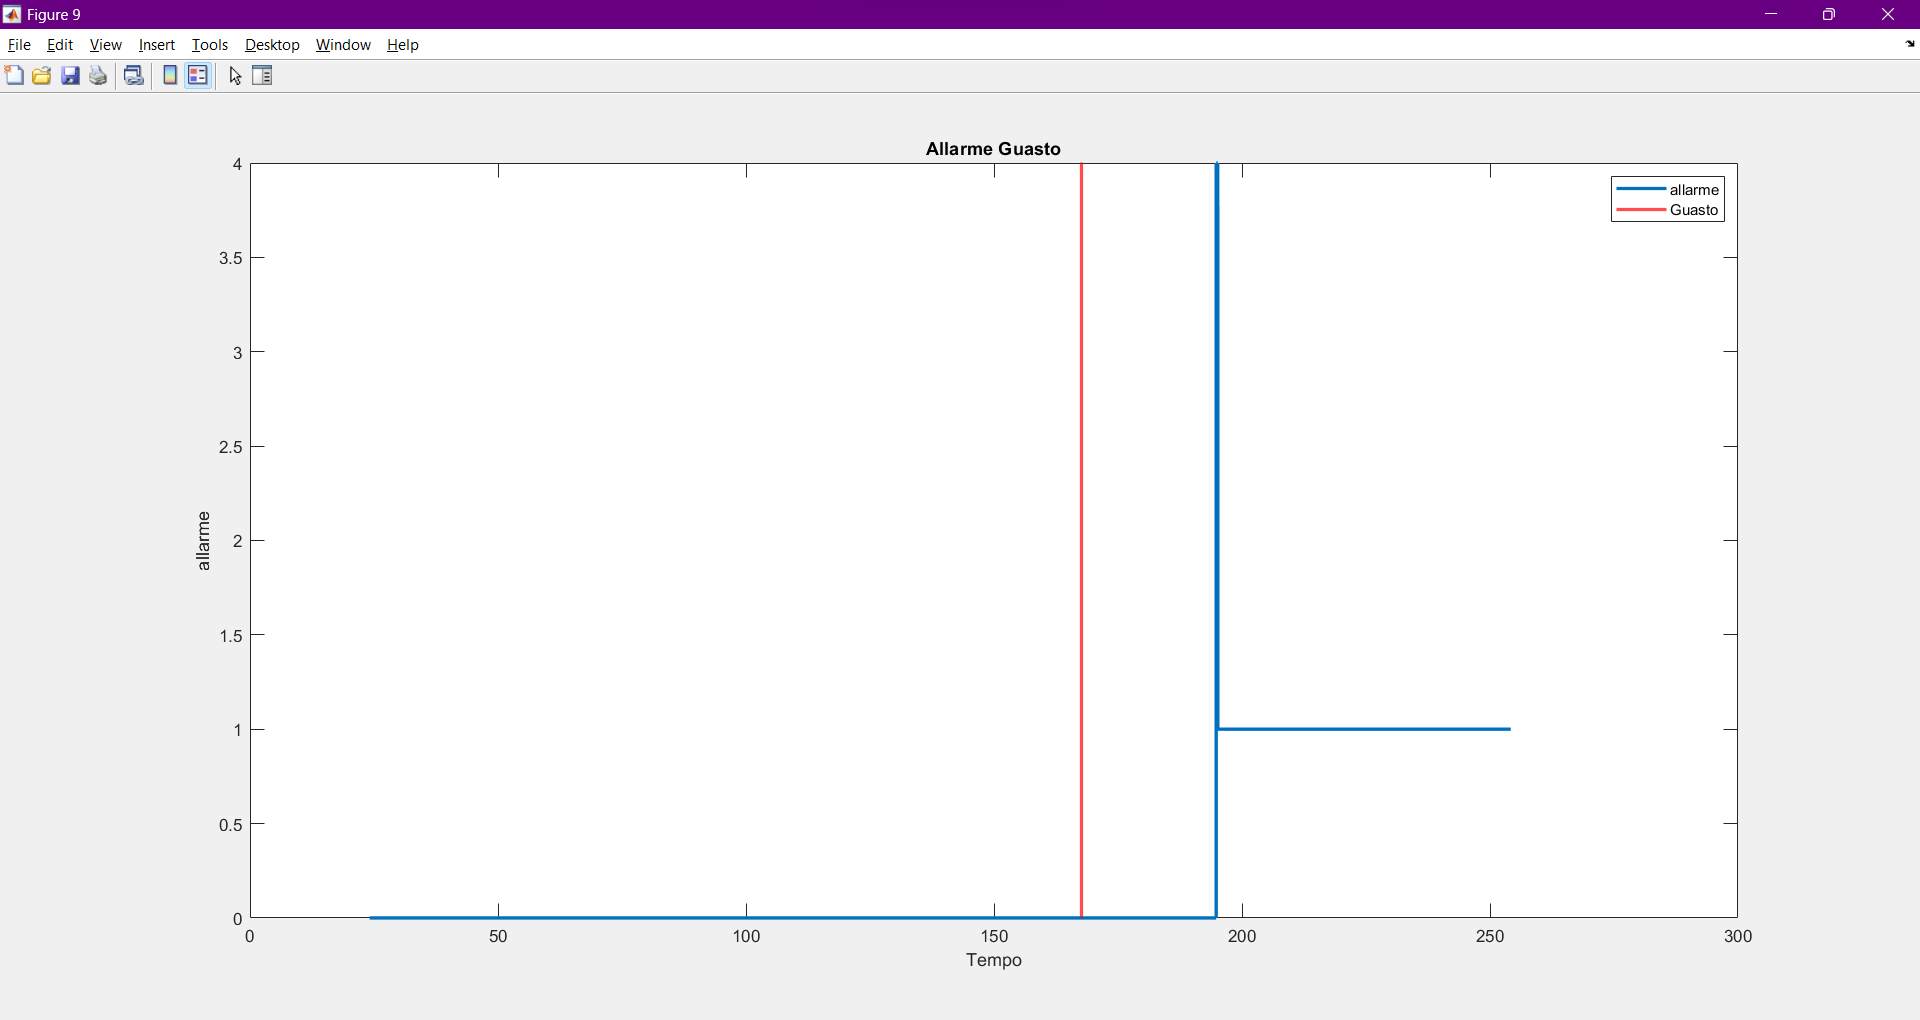
\includegraphics[width=\textwidth]{files/images/path_soglia_fissa1 (3).png}
    \caption{Allarmi del test volo con guasto su potenza motore del 20\% su motore 1}
    \label{Allarmi del test volo con guasto su potenza motore del 20\% su motore 1}
\end{figure}
\noindent

\begin{figure}[H]
    \centering
    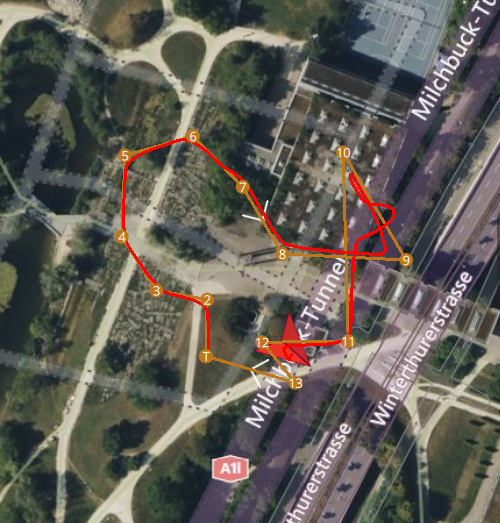
\includegraphics[width=0.5\textwidth]{files/images/path_soglia_fissa2 (1).png}
    \caption{Andamento del drone del test volo con guasto su potenza motore del 20\% su motore 2}
    \label{Risultato volo con guasto su potenza motore del 20\% su motore 2}
\end{figure}
\noindent

\begin{figure}[H]
    \centering
    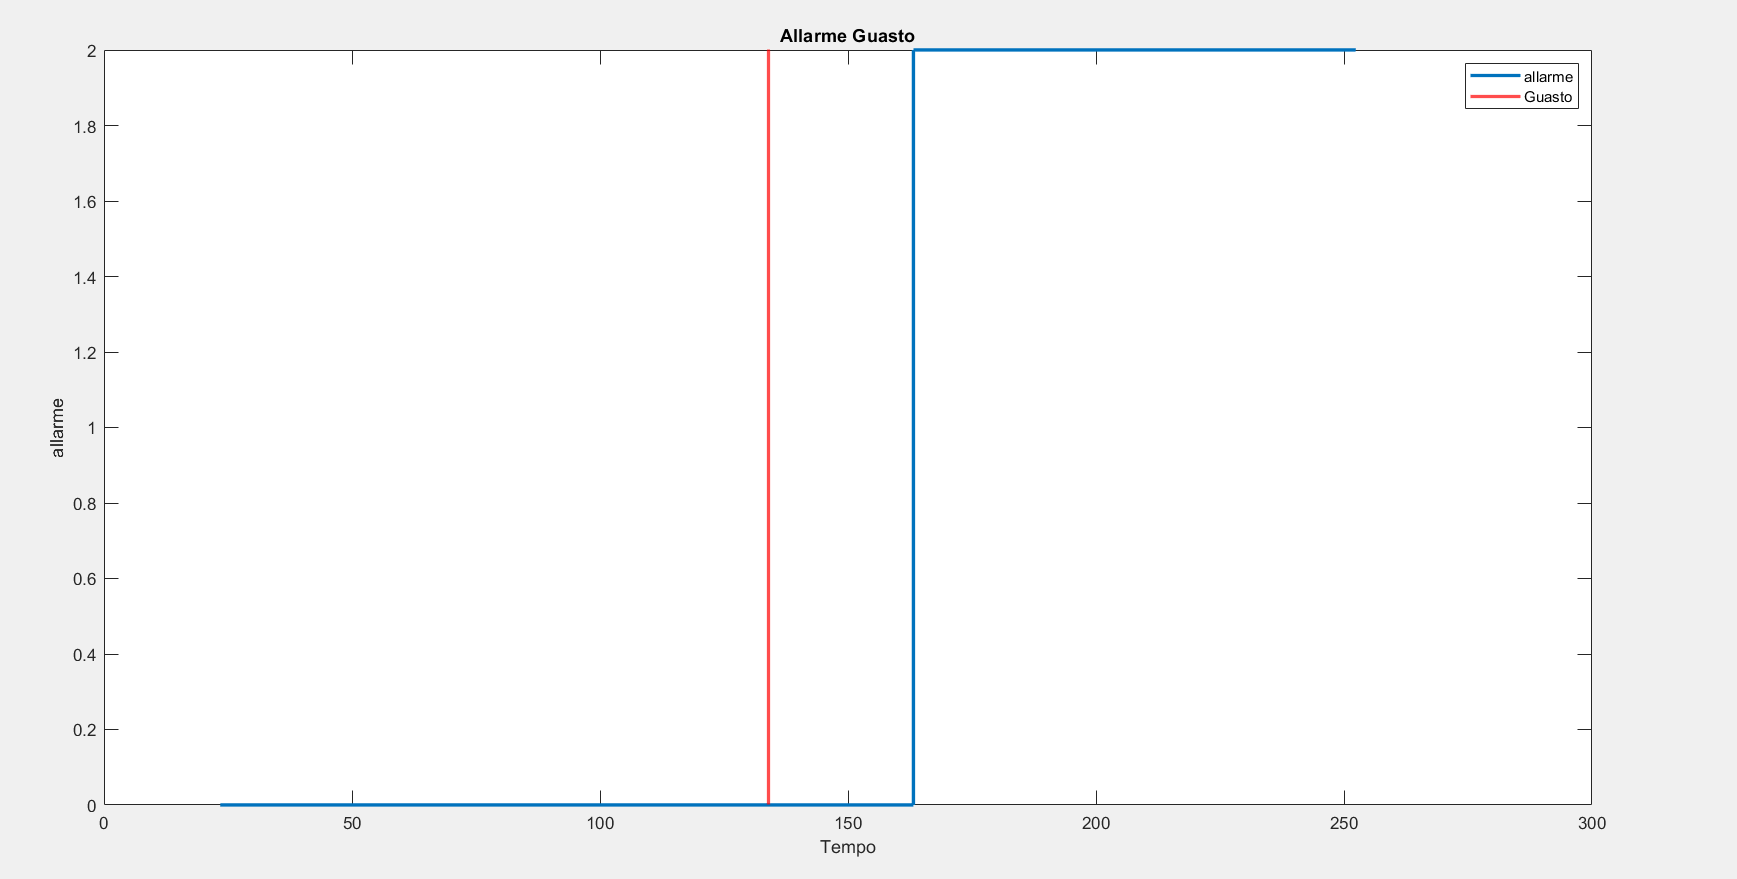
\includegraphics[width=\textwidth]{files/images/path_soglia_fissa2 (2).png}
    \caption{Allarmi del test volo con guasto su potenza motore del 20\% su motore 2}
    \label{Allarmi del test volo con guasto su potenza motore del 20\% su motore 2}
\end{figure}
\noindent

\begin{figure}[H]
    \centering
    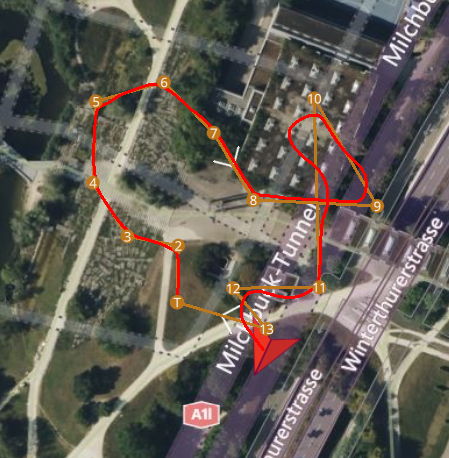
\includegraphics[width=0.5\textwidth]{files/images/path_soglia_fissa3 (2).png}
    \caption{Andamento del drone del test volo con guasto su potenza motore del 20\% su motore 3}
    \label{Risultato volo con guasto su potenza motore del 20\% su motore 3}
\end{figure}
\noindent

\begin{figure}[H]
    \centering
    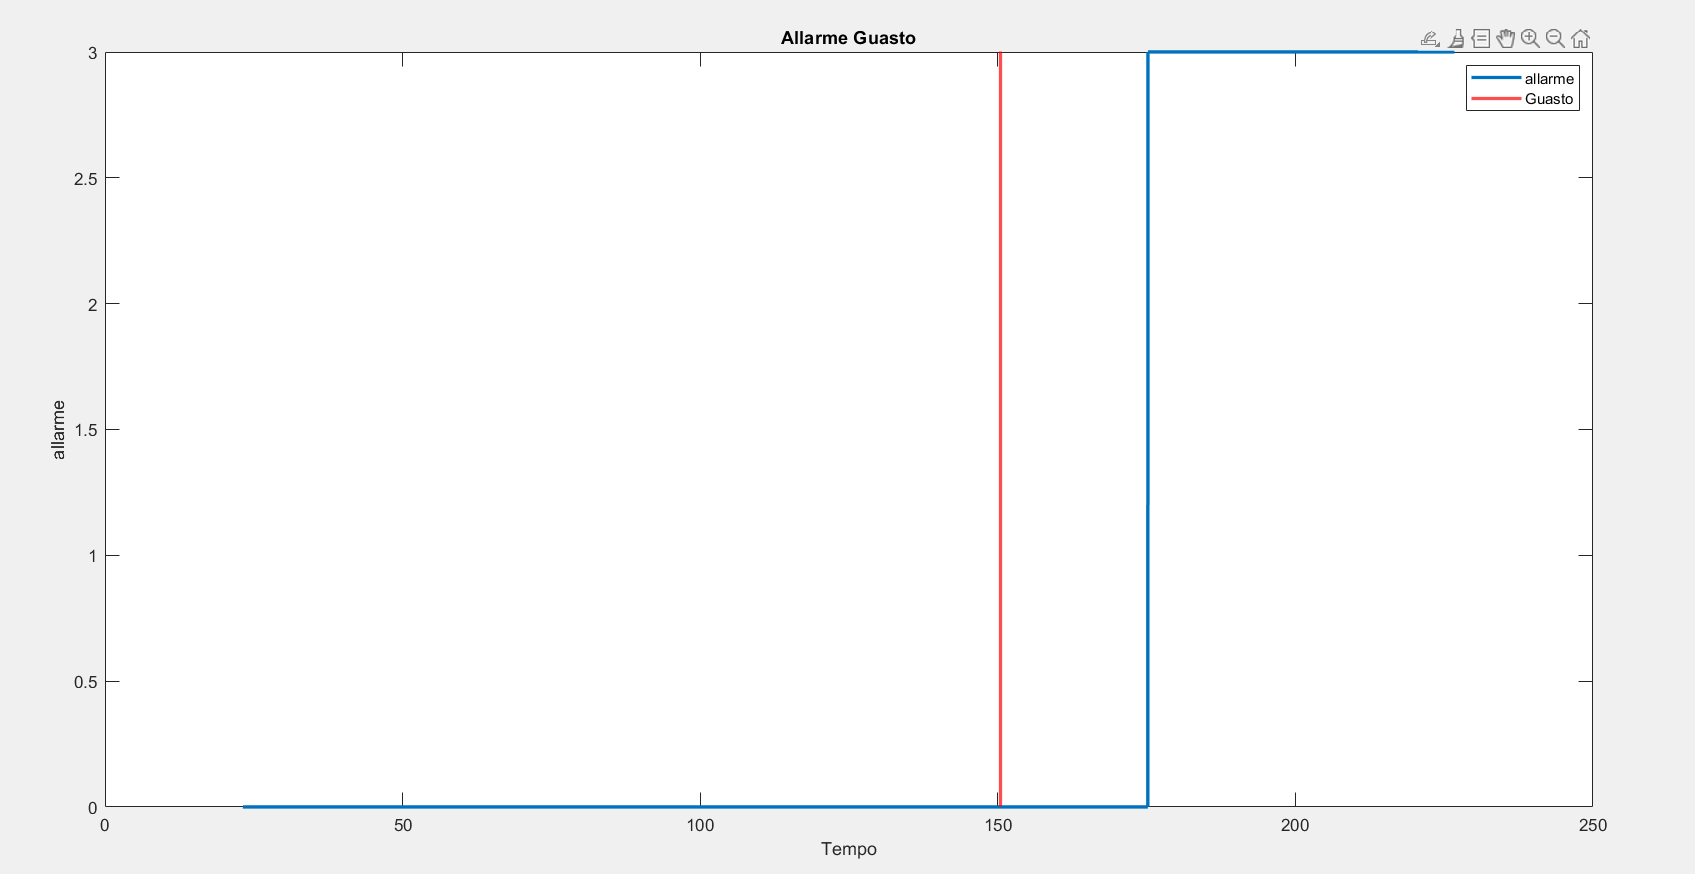
\includegraphics[width=\textwidth]{files/images/path_soglia_fissa3 (1).png}
    \caption{Allarmi del test volo con guasto su potenza motore del 20\% su motore 3}
    \label{Allarmi del test volo con guasto su potenza motore del 20\% su motore 3}
\end{figure}
\noindent

\begin{figure}[H]
    \centering
    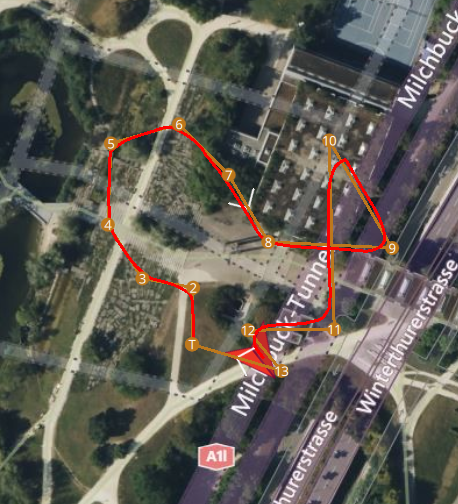
\includegraphics[width=0.5\textwidth]{files/images/path_soglia_fissa4 (2).png}
    \caption{Andamento del drone del test volo con guasto su potenza motore del 20\% su motore 4}
    \label{Risultato volo con guasto su potenza motore del 20\% su motore 4}
\end{figure}
\noindent

\begin{figure}[H]
    \centering
    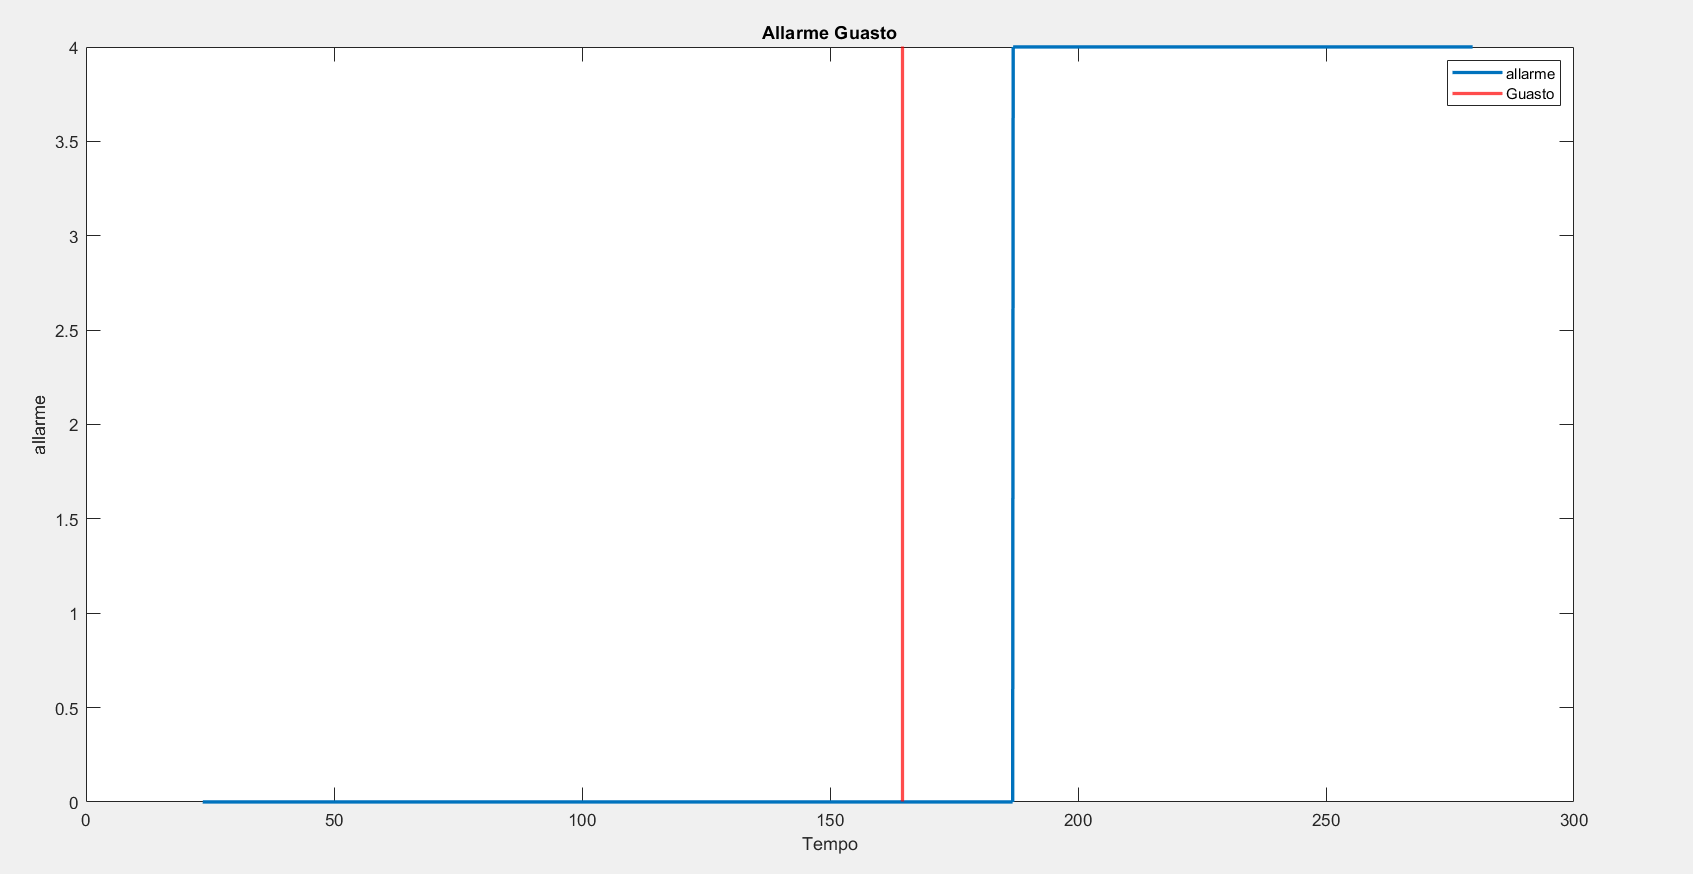
\includegraphics[width=\textwidth]{files/images/path_soglia_fissa4 (1).png}
    \caption{Allarmi del test volo con guasto su potenza motore del 20\% su motore 4}
    \label{Allarmi del test volo con guasto su potenza motore del 20\% su motore 4}
\end{figure}
\noindent

\section{Rilevamento dei Guasti con Soglia Adattiva}

Nella fase successiva del nostro studio, abbiamo esplorato un approccio di rilevamento dei guasti con soglia adattiva. Questo metodo si basa sull'utilizzo degli errori degli angoli di pitch e roll, analogamente alla sezione precedente.
\\
La soglia adattiva è stata calcolata nel seguente modo:
\begin{equation}
\text{PitchThreshold} = 0.1 + \left(\text{mean}(PitchBufferDes) \times \text{mean}(PitchBuffer)\right)
\end{equation}
\begin{equation}
\text{RollThreshold} = 0.1 + \left(\text{mean}(RollBufferDes) \times \text{mean}(RollBuffer)\right)
\end{equation}
\noindent
Queste equazioni rappresentano il calcolo delle soglie adattive per il rilevamento dei guasti, dove il valore di partenza 0.1 viene aggiunto a un contributo basato sul prodotto delle medie degli errori di pitch e roll e dei valori desiderati di pitch e roll.
\\
Per implementare il rilevamento dei guasti con soglia adattiva, abbiamo sviluppato un algoritmo che regola dinamicamente le soglie di rilevamento in base alla variazione del valore desiderato di angolo. La struttura blocchi all'interno di Quadcopter\_ControllerWithNavigation è simile a quello inserito per la soglia fissa (Fig. \ref{Rilevamento guasti con soglia adattiva Quadcopter\_ControllerWithNavigation}).
\\
\begin{figure}[H]
    \centering
    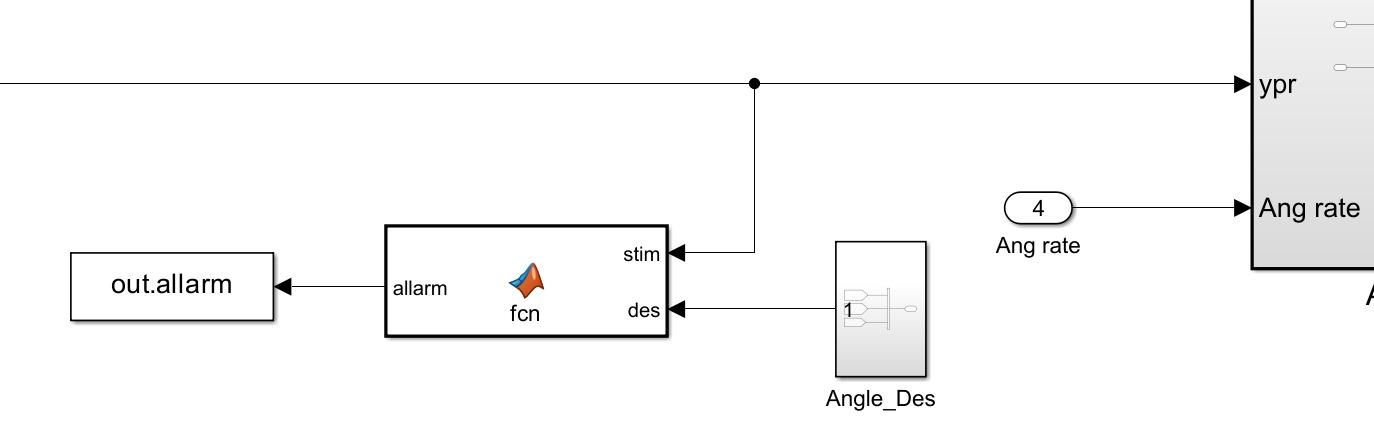
\includegraphics[width=0.5\textwidth]{files/images/WhatsApp Image 2024-03-15 at 18.28.16.jpeg}
    \caption{Rilevamento guasti con soglia adattiva Quadcopter\_ControllerWithNavigation}
    \label{Rilevamento guasti con soglia adattiva Quadcopter\_ControllerWithNavigation}
\end{figure}
\noindent
Il codice all'interno della MATLAB function è il seguente.
\begin{lstlisting}[language=Matlab, caption={Descrizione del codice}, label={lst:codice_matlab}]
function allarm = fcn(stim, des)
    persistent PitchBuffer RollBuffer 
    PitchBufferDes RollBufferDes
    if isempty(PitchBuffer)
        PitchBuffer = zeros(1, 500);
        RollBuffer = zeros(1, 500);
        PitchBufferDes = zeros(1, 500);
        RollBufferDes = zeros(1, 500);
    end

    % Calcolo gli errori di Pitch e Roll
    Pitch_Error = des(2) - stim(2);
    Roll_Error = des(3) - stim(3);

    % Per evitare che la media dia errore per i NaN, 
    sostituisco con 0
    if(isnan(Pitch_Error) && isnan(Roll_Error))
       Pitch_Error = 0;
       Roll_Error = 0;
    end

    % Aggiorna i buffer
    PitchBuffer = [PitchBuffer(2:end), Pitch_Error];
    RollBuffer = [RollBuffer(2:end), Roll_Error];
    PitchBufferDes = [PitchBufferDes(2:end), des(2)];
    RollBufferDes = [RollBufferDes(2:end), des(1)];;

    % Soglia Adattiva 
    PitchThreshold = 0.1 + 
    (mean(PitchBufferDes)*mean(PitchBuffer));
    RollThreshold = 0.1 + 
    (mean(RollBufferDes)*mean(RollBuffer));

    % Guasto Motore 1 del -20%
    if (mean(PitchBuffer) > PitchThreshold && 
    mean(RollBuffer) < -RollThreshold)
        allarm = 1;
    % Guasto Motore 2 del -20%
    elseif (mean(PitchBuffer) < -PitchThreshold && 
    mean(RollBuffer) > RollThreshold)
        allarm = 2;
    % Guasto Motore 3 del -20%
    elseif (mean(PitchBuffer) > PitchThreshold && 
    mean(RollBuffer) > RollThreshold)
        allarm = 3;
    % Guasto Motore 4 del -20%
    elseif (mean(PitchBuffer) < -PitchThreshold && 
    mean(RollBuffer) < -RollThreshold)
        allarm = 4;
    else
        allarm = 0;
    end
end
\end{lstlisting}
\noindent
Vengono inizializzati quattro buffer per registrare gli errori di pitch e roll, così come i valori desiderati di pitch e roll. Questi buffer vengono utilizzati per calcolare le medie degli errori nel tempo. Viene calcolato l'errore tra gli angoli desiderati e quelli stimati di pitch e roll. Gli errori di pitch e roll vengono aggiunti ai buffer e gli elementi più vecchi vengono rimossi per mantenere una dimensione fissa dei buffer. Le soglie adattive per il rilevamento dei guasti vengono calcolate in base alle medie degli errori di pitch e roll e dei valori desiderati di pitch e roll. Le soglie adattive si adattano dinamicamente alle variazioni nelle condizioni di volo. Viene eseguito il rilevamento dei guasti confrontando le medie degli errori di pitch e roll con le soglie adattive. Se le condizioni corrispondono a un guasto specifico, viene attivato l'allarme corrispondente al motore interessato.
\\
Durante la fase di volo, il nostro algoritmo monitora costantemente gli errori degli angoli di pitch e roll e aggiorna le soglie di rilevamento.
\\
\begin{figure}[H]
      \centering
      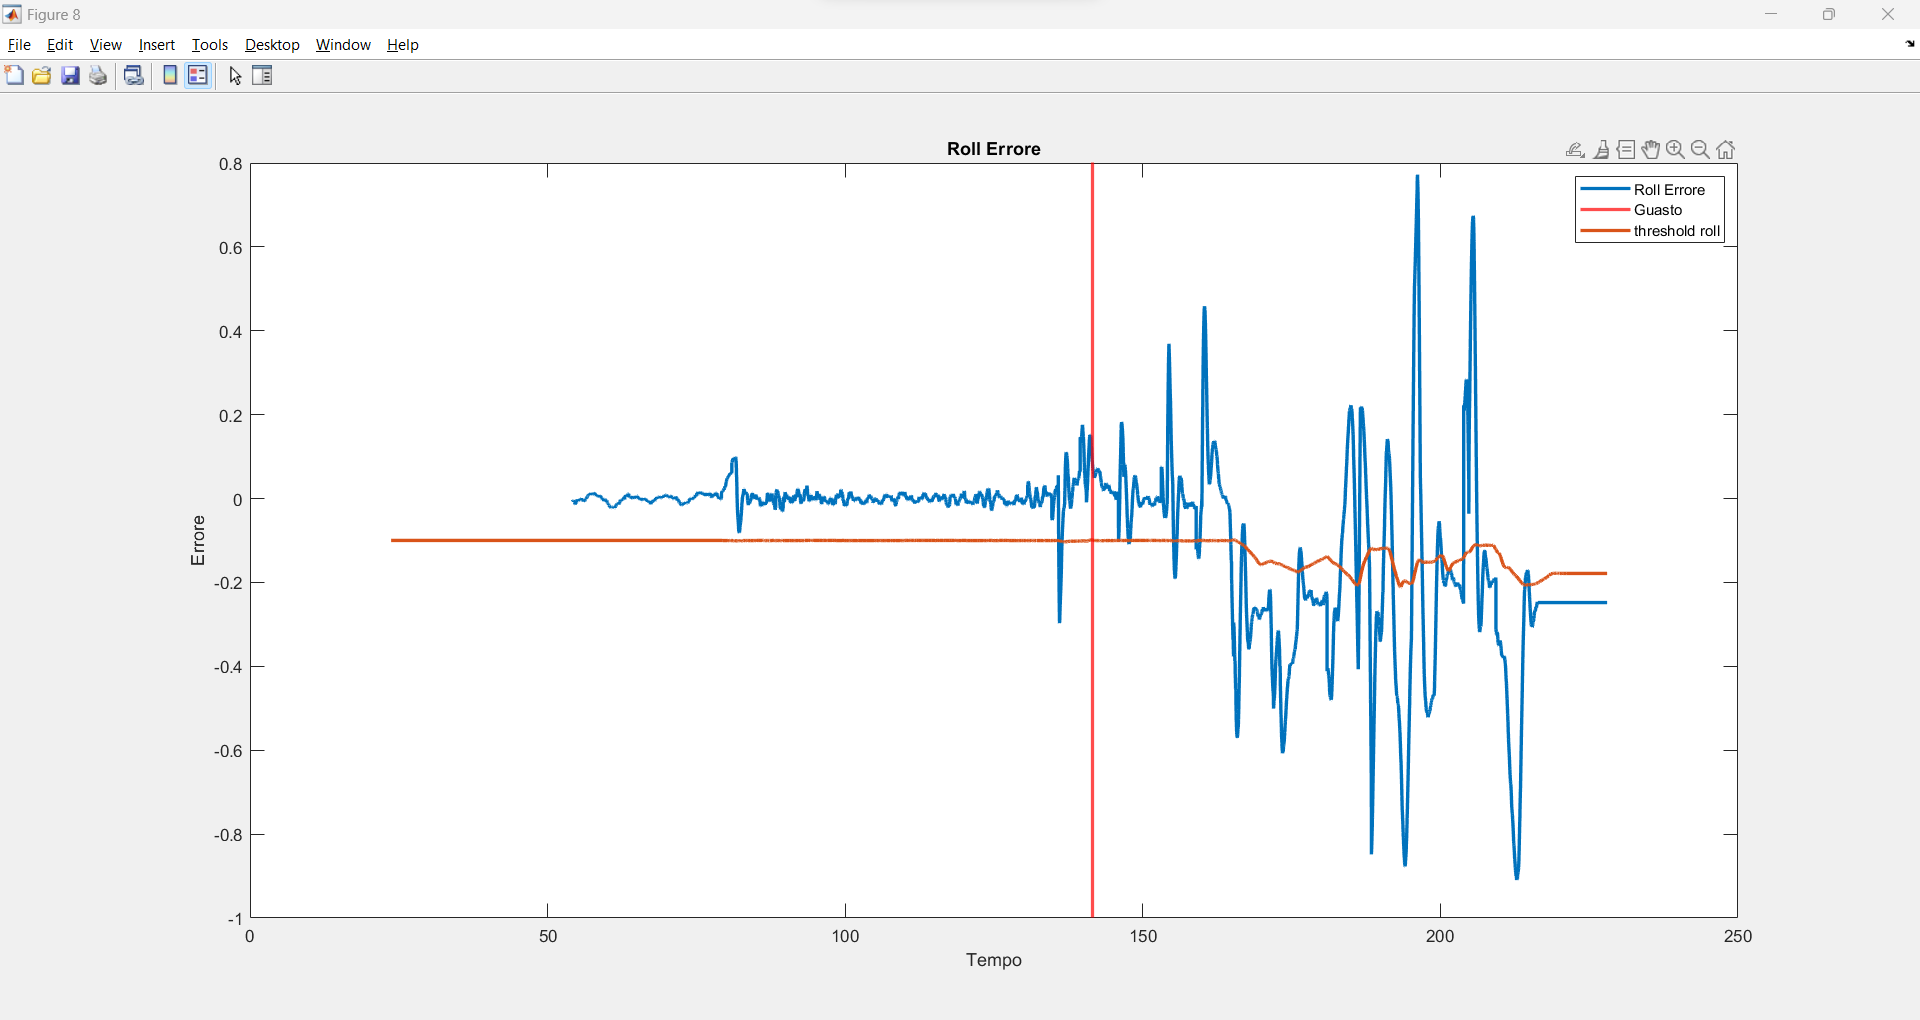
\includegraphics[width=\linewidth]{files/images/soglia_adattiva_roll.png} % Imposta la larghezza dell'immagine al 50% della larghezza del testo
      \caption{Soglia Adattiva Roll} % Didascalia sotto l'immagine
      \label{fig:Soglia adattiva Roll} % Etichetta per fare riferimento all'immagine nel testo
\end{figure}%
\begin{figure}[H] % Definisci la larghezza della seconda minipage (50% della larghezza della pagina)
        \centering
        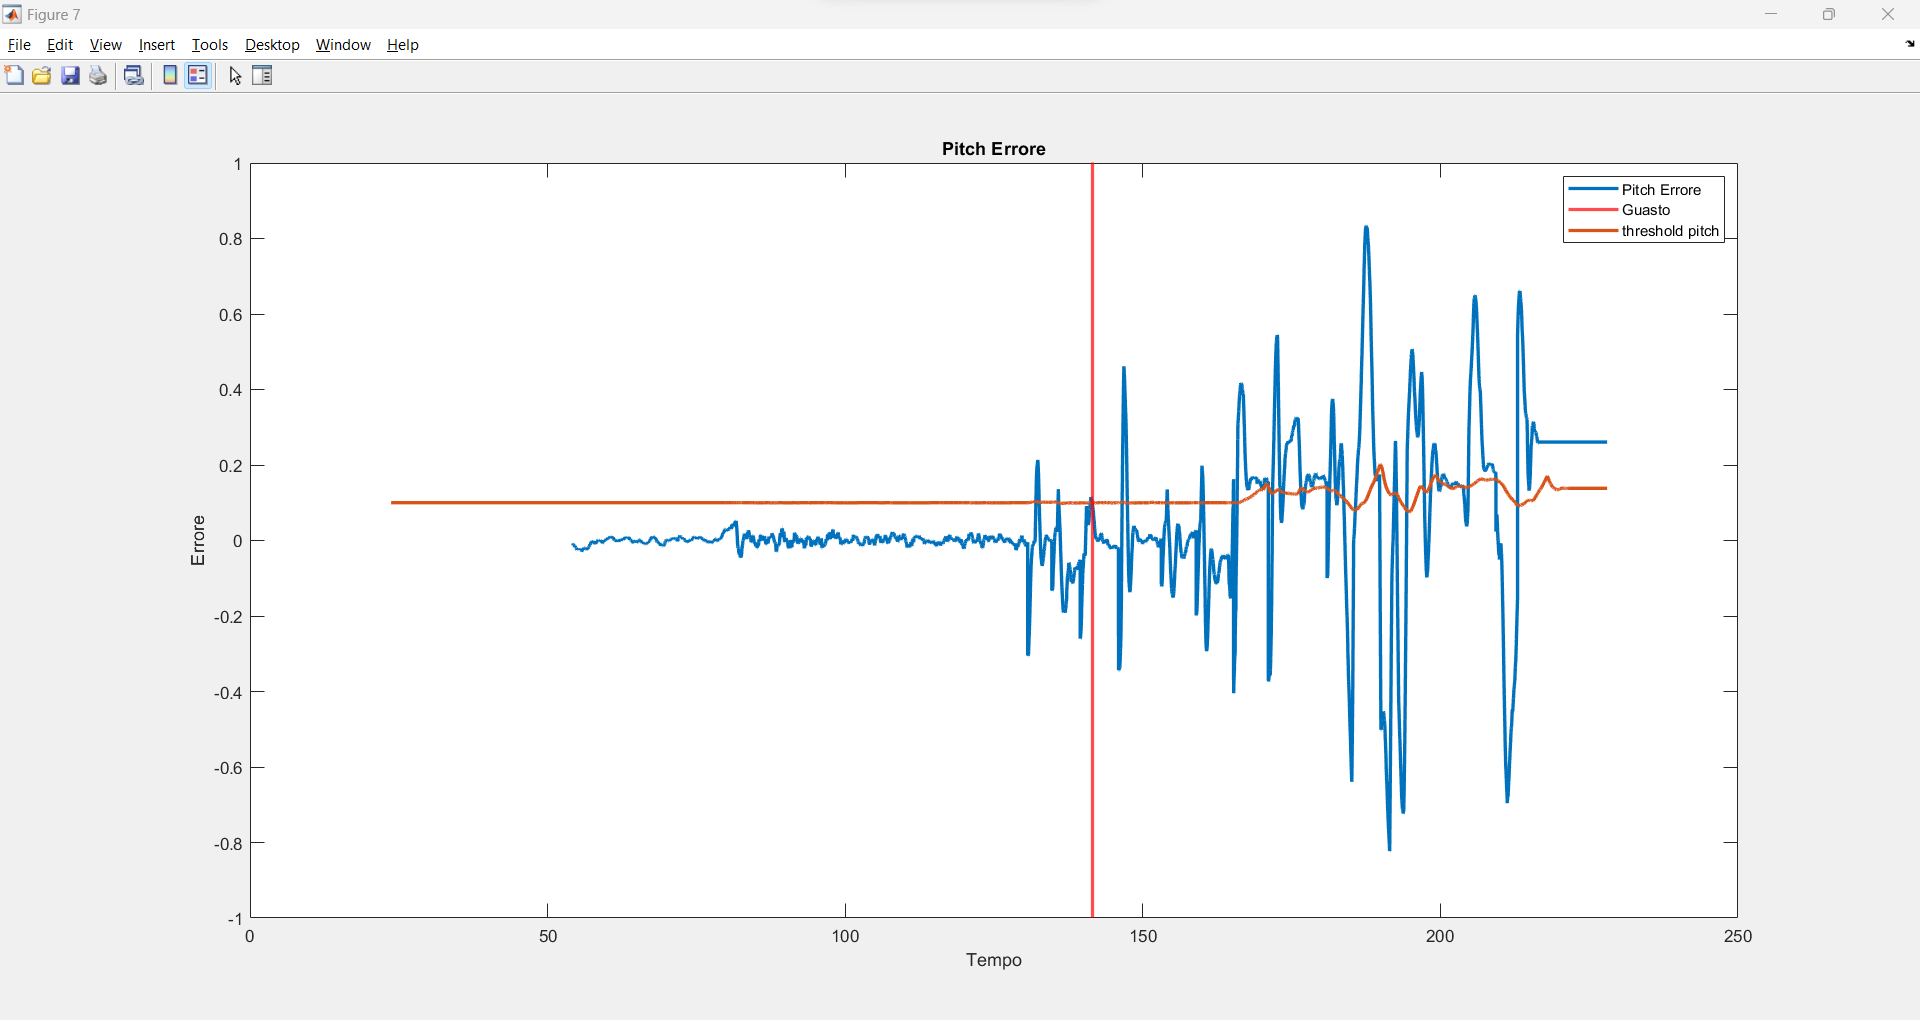
\includegraphics[width=\linewidth]{files/images/soglia_adattiva_pitch.png} % Imposta la larghezza dell'immagine al 50% della larghezza del testo
        \caption{Soglia Adattiva Pitch} % Didascalia sotto l'immagine
      \label{fig:Soglia Adattiva Pitch} % Etichetta per fare riferimento 
\end{figure}
\begin{figure}[H]
    \centering
    \includegraphics[width=\textwidth]{files/images/allarmi_soglia_adattiva.png}
    \caption{Allarmi rilevati con soglia adattiva con perdita di potenza del 20\% sul motore 1}
    \label{Allarmi soglia adattiva}
\end{figure}
\noindent
I risultati preliminari ottenuti utilizzando il rilevamento dei guasti con soglia adattiva sono simili a quelli con soglia fissa con buffer (Fig. \ref{Allarmi soglia adattiva}). Abbiamo osservato che il guasto viene rilevato dopo una prima curva che il drone effettua.
\\
Ulteriori studi e test sono necessari per valutare completamente le prestazioni e l'efficacia del rilevamento dei guasti con soglia adattiva, ma i risultati preliminari indicano un potenziale significativo per il rilevamento guasti sui motori.
